%!TEX root = ../report.tex

\chapter{Popov-Vereshchagin hybrid dynamics solver for operational-space control}

%A hybrid dynamics algorithm is a generalization of forward and inverse dynamics problem [Featherstone, 2008]: in which we are aware of the forces at some joints, and accelerations in the remaining, and the task is to calculate the unknown forces and accelerations. Hybrid dynamics is also the major algorithm for the posture control[Khatib et al., 1999] of mobile manipulators and humanoid robots, since such tasks typically require specifications of motion and/or force constraints on the end-effectors and other segments, but also specifications/constraints on postures.\cite{Shaki}
\par
%In-order to model and control the motion a robot, there is a requirement of equations of motion with robot end effector mechanism, equations that relate the control moments and forces at the joints with the position velocity and acceleration which takes complete dynamics taken into account.\cite{Popov-vereschagin}. There are three different methods to obtain solution to the dynamics problems. They are methods based on Newton-Euler equations, methods based on Lagrange equations and methods based on the variational principles of mechanics. Methods-based on Gauss principle of least constraints and its various modifications belong to the third category. 
\par
%The robot dynamics literature is extremely abundant and rich. They followed from the historical general dynamics work by [Newton, 1871, Euler, 1776, Lagrange, 1867, Gauss, 1829] (the latter’s minimum principle being further developed by [Gibbs, 1879, Hertz, 1894] and [Appell, 1899]), to general multi-body dynamics [Gantmacher, 1975, Roberson and Schwertassek, 1988, Wittenburg, 1977], and leading to robot-specific dynamics literature, first as “order $N^3$” $(O(N^3))$ algorithms [Hooker and Margulies, 1965, Lilov and Wittenburg, 1977, Luh et al., 1980a, Roberson and Wittenburg, 1966], and later as $O(N)$ (“order N”) algorithms [Vereshchagin, 1974, Popov et al., 1978, Featherstone, 1983], where N is the number of degrees of freedom in the kinematic chain of the robot.
\section{Robot Control and Optimizations Techniques:}
The software architectures which help in the development of the framework designed for task control faces an issue called constrained optimization problem. i.e., it has to be able to resolve constraints imposed by task definition. The related work section discusses on OCP.\cite{Reference to section related work}. There are different methods to solve for the optimal control problem:\cite{shakhimardanov2015} dynamic programming, indirect methods and direct methods.
\par
	The implementations of these numerical techniques into an algorithm or software representation is called a solver. These solvers are categorized as domain specific solvers and domain independent solvers. Examples of domain specific solvers are: Newton-Euler, which is an recursive inverse dynamics solver.  If the domain knowledge is the known then it helps in efficient calculation.\cite{shakhimardanov2015}. The mathematical representation based on acceleration scheme(domain independent) which takes into consideration of dynamics of robots is given by \cite{shakhimardanov2015}
	$$M(q)\ddot{q} = \tau(q,\dot{q})$$
	where $M(q)$ is the inertia matrix. After the specification of the constraints, the equation is represented as according to\cite{shakhimardanov2015}
	$$M(q)\ddot{q} = \tau_{a}(q) - \tau_{c}(q) - C(q,\dot{q})$$
	$$h(q) = 0$$
where $\tau_{a}(q)$ is the input forces $\tau_{c}(q)$ denote constraint forces, $C(q,\dot{q})$ denote bias forces and $h(q) = 0$ represent holonomic position constraints.\cite{shakhimardanov2015}
These equations require the motion equations of end effector, which also considers the forces and inertia at the joints. Mass and other inertial properties are accounted for the elements along with position, velocities, acceleration etc. \cite{vereshchagin1989modeling}
\section{Solver Description}
The main functionality of the solver is to compute control commands which will solve for the constraints imposed on the end effector by the task definition. This hybrid dynamics algorithm computes required control commands based on the defined constraints, the robot model, the feedforward joint torques and the external forces applied onto each segment of robot system.\cite{vereshchagin1989modeling}. This solver also prioritizes acceleration constraints over force constraints.
A general mathematical representation of this above mentioned problem is given as the expanded matrix form of the equation[].\cite{}
$$\begin{bmatrix}
M(q) & J_{c}^{T}(q)\\
J_{c}(q) & 0
\end{bmatrix}
\begin{bmatrix}\\
\ddot{q} \\
\lambda
\end{bmatrix} = 
\begin{bmatrix}
\tau_{a}(q) - C(q,\dot{q}) \\ 
\hat{b}{(q,\dot{q})}
\end{bmatrix}$$
where $J_{c}(\ddot{q}) = \hat{b}(q,\dot{q})$ is the second order derivative of the holonomic path constraint h(q) = 0 , $J_{c}$ is the constraint matrix, $\lambda$ is the vector of Lagrange multipliers with the relation to the constraint forces being $\tau_{c} = J_{c}^{T}\lambda$, $C(q,\dot{q})$ and $\tau_{a}$ are bias forces and joint space input forces, respectively.\cite{featherstone2014rigid}
\par
There have been different methods evaluated for many years which allow and find solutions numerically to the dynamic problems through initial procedures or by building dynamic models of kinematic chains.\cite{vereshchagin1989modeling}. There are three popular methods in three different groups, among them gauss principle of least constraint belongs to variational principles of mechanics.\cite{vereshchagin1989modeling}"The guass's principle states that the true motion can be represented by the minimum of a convex function(concave downward or upward) which is unique and is defined by linear equations and inequalities."\cite{vereshchagin1989modeling}. That means that the acceleration which minimizes that acceleration energy is the real/true motion in the context of Vereshchagin solver. Similary, Popov-Vereshchagin algorithm solves for the external constraints which are of type acceleration which computes the control commands such as motion and forces linked to kinematic chain. The solution proposed to this constrained optimization problem is by improvising the equation as in \cite{vereshchagin1989modeling}\cite{shakhimardanov2015}:
$$A_{N}^{T}\ddot{X}_{N} = b_{N}$$.
Such optimization problem is known as Gauss’s principle of least constraint.\cite{shakhimardanov2015}. The Gauss function which is minimized is thus given as \cite{vereshchagin1989modeling}:
$$ Z = \sum_{i=0}^{N}\frac{1}{2}\ddot{X}_{i}^{T}H_{i}\ddot{X}_{i} + U^{T}_{i}\ddot{X}_{i}+ \sum_{j=1}^{N}\frac{1}{2}d_{j}\ddot{q}_{j}^{2} - Q_{j}\ddot{q}_{j}$$
where Z is called as the Zwang Degree of constraint, $H_{i}$ is the inertial matrix of size $n \times n $ where n is the dimension of matrix, $U_{i}$ represents the effects of external forces, Coriolis and centrifugal forces, which is collectively called as bias force which is a vector of size $n\times 1$ and $Q_{j}$ the feedforward joint torques.\cite{vereshchagin1989modeling}. As mentioned above this Gauss function is minimized subjected to the acceleration constraints, which is represented as:
$$min  Z(\ddot{q}) $$
constrained to : $$ a_{i+1} = {^{i+1}X_{i}} a_{i} + S_{i}\ddot{q}_{i+1}+ C_{i}$$
$$A_{N}^{T}a_{N} = b_{N}$$
where $a_{i+1}$ is represented as $\ddot{X}_{i+1}$ which includes both linear and angular accelerations for particular links.Expression consisting $A_{N}$ is a matrix of unit constraint forces. $b_{N}$ matrix denotes the vector of acceleration energy for segment N. In-order to provide extension of the solver in considering acceleration constraints on segments, according to the principle of Bellman's optimality\cite{bellman2013dynamic}the equation[] can be represented as:
$$min  Z(\ddot{q},\nu)  = \sum_{i=0}^{N}\frac{1}{2}\ddot{X}_{i}^{T}H_{i}\ddot{X}_{i} +  \sum_{j=1}^{N}\frac{1}{2}d_{j}\ddot{q}_{j}^{2} - Q_{j}\ddot{q}_{j} + \nu^{T}A_{N}^{T}\ddot{X}_{i}$$
"The above equation represents the search for the minimum of Lagrange function"\cite{shakhimardanov2015}\cite{lagrange1853mecanique}, where $\nu$ represents the Lagrange multiplier.
%The linear-time hybrid dynamics algorithm \cite{Compothe trsable Robot Motion Stack} allows to deal with the motion constraints on the segments at the acceleration level, and the specification of each constraint can be only partial, i.e., allowing one or more degrees of constraint to be left unspecified [Vereshchagin, 1989]. It computes the magnitudes of the constraint forces that are caused by the imposed Cartesian acceleration constraints based on the Gauss principle of least action \cite{Guass 1829} as the function(cost) to optimize.
\newpage
\par 
%write about gauss function minimization.
\section{Brief overview of Vereshchagin solver}
\begin{itemize}
	\item The input requirements to the solver are : The robot model, joint angles and joint velocities at the current time instant, the feedforward joint torque, the external forces applied to individual segments and $A_{N}$ is the desired constraint(unit force) matrix and $b_{N}$ is the desired bias acceleration (energy) term.
	\item Since the hybrid dynamics problem is a general case of both inverse and forward problems and computes either motions or forces of a kinematic chain depending on the input output causality at a particular joint constraint. i.e it computes the desired control torques, the accelerations resulting from those torques. 
\end{itemize}
%In the sweeps, the variables q,$\dot{q}$, $\ddot{q}$, $\tau_{a}$ at each joint are associated with their spatial counterparts X, $\dot{X}$, $\ddot{X}$, F at each segment., similarly use inward recursion for force and spatial inertia, \cite{shakhimardanov2015}.Thus these recursive operations are also known as an outward and inward computational sweeps on the kinematic chain.\cite{shakhimardanov2015}.
\par
The Vereshchagin algorithm is a three pass/sweep algorithm. These sweeps are recursive over kinematic tree. The first is the outward sweep that calculates the propagation of pose, velocity and bias terms from the root of the robot to the leafs. Then, comes the inward sweep that calculates the articulated-body inertia dependent acceleration which can be caused of external forces represented as, torques on the joints and bias forces along with computation of acceleration energy contributions generated by unit constraint forces. The last sweep is the outward sweep again, which calculates the end result of joint torques and Cartesian accelerations for each segment. 
\par 
We can customize and calculate only specific terms of dynamics by setting certain inputs to zero.\cite{featherstone2014rigid} For eg, if there are no contributions from the external forces in the outward sweep, then the bias term for acceleration expects to be only change from Coriolis and centrifugal effects.
In the inward sweep, articulated body inertia and forces are calculated as result of summation of apparent inertias and apparent forces.\cite{featherstone2014rigid}.
This hybrid dynamics solver has the run time complexity of linear time recursion, i.e, $O(n)$. 
%i.e calculate the velocity-product accelerations, these bias accelerations representing change in link velocities assume that no external forces are being applied on that particular body. This inturn indicates that the existence of this acceleration is influenced by Coriolis and centrifugal effects only, if we set gravity and external force terms all to zero, then the accelaration is affected only by the Coriolis and centrifugal terms. \cite{Featherstone}. The rigid body bias forces are made use in later passes.
%The next step is to calculate the articulated-body inertias and bias forces along with computation of acceleration energy contributions generated by unit constraint forces. "Ij a and paj have one more interesting property: they express the force across a joint as a function of the parent body’s acceleration, whereas IAj and pA j express this same force as a function of the child’s acceleration."(change it)
\newpage
\begin{algorithm}[H] \label{alg1}
	The formulation of algorithm can be given as \cite{popov78, algoVer, shakhimardanov2015}:\\
	\SetAlgoLined
	\SetKwInOut{Input}{Input}
	\SetKwInOut{Output}{Output}
	\Input{\ $\mathbf{Robot \ model, \ q, \ \dot{q}, \ \mathbf{\mathlarger{\mathlarger{\tau}}}, \ \ddot{X}_0, \ F_{ext}, \ A_N, \ b_N}$}
	\Output{\ $\mathbf{\mathlarger{\mathlarger{\tau_{\textbf{control}}}}}, \ \mathbf{ \ddot{q}, \ \ddot{X}}$}
	
	\SetKwBlock{Begin}{begin}{end}
	\Begin{
		{// Outward sweep of position, velocity and bias components}\\
		\For{$\mathbf{i \ = \ 0 \ \ to \ \ N-1}$}{
			${}^{i+1}_{i}X = ({}^{d_i}_{i}X \ \  {}^{i+1}_{d_i}X(q_i))$\; \label{alg:pose}
			\vspace{1mm}
			${\dot{X}_{i+1} = {^{i+1}X_{i}} \dot{X}_i + S_{i+1} \dot{q}_{i+1}}$\; \label{alg:velocity}
			\vspace{1mm}
			${\ddot{X}_{bias,i+1} = {\dot{X}_{i+1}} \times S_{i+1} \dot{q}_{i+1}}$\; \label{alg:bias_acc}
			\vspace{1mm}
			${F_{bias,i+1} = {\dot{X}_{i+1}} \times^* I_{i+1} \dot{X}_{i+1}- {^{i+1}X_{0}^*} \ {F}^{ext}_{0,i+1}}$\; \label{alg:bias_force}
			\vspace{1mm}
			${{F}^{A}_{bias,i+1} = F_{bias,i+1}}$\; \label{alg:bias_force_A}
			\vspace{1mm}
			${I_{i+1}^A = I_{i+1}}$\; \label{alg:I_A}
		}
		\vspace{2mm}
		{// Inward sweep of inertia, force and acceleration energy contributions}\\
		\For{$\mathbf{i \ =  \ N-1  \ \ to \  \ 0}$}{
			${D_{i+1} = d_{i+1} + S_{i+1}^T I_{i+1}^A S_{i+1} }$\; \label{alg:sum_inertia}
			\vspace{2mm}
			${P_{i+1}^A = 1 - I_{i+1}^AS_{i+1} D_{i+1}^{-1} S_{i+1}^{T}}$\; \label{alg:P}
			\vspace{2mm}
			${I_{i+1}^a = P_{i+1}^A I_{i+1}^A}$\;
			\label{alg:I_a}
			\vspace{2mm}
			${I_i^A = I_i^A + \sum{^{i}X_{i+1}^T} I_{i+1}^a {^{i}X_{i+1}}}$\; \label{alg:I_A2}
			\vspace{1mm}
			${F_{bias,i+1}^a = P_{i+1}^A F_{bias,i+1}^A + I_{i+1}^AS_{i+1} D_{i+1}^{-1} \tau_{i+1}+ I_{i+1}^a\ddot{X}_{bias,i+1}}$\; \label{F_bias_a}
			\vspace{2mm}
			${F_{bias,i}^A = F_{bias,i}^A + \sum{^{i}X_{i+1}^*} F_{bias,i+1}^a}$\; \label{F_bias_A}
			\vspace{2mm}
			${A_i = {^{i}X_{i+1}^T} P_{i+1}^A A_{i+1}}$\;  \label{alg:A_i}
			\vspace{2mm}
			${U_i = U_{i+1} + A_{i+1}^T \{\ddot{X}_{bias,i+1} + S_i D^{-1}_i(\tau_{i+1} - S_i^T(F_{bias,i+1}^A + I_{i+1}^a \ddot{X}_{bias,i+1}))\}}$\; \label{alg:U_i}
			\vspace{-4mm}
			${\mathcal{L}_i = \mathcal{L}_{i+1} - A_{i+1}^T S_{i+1}D^{-1}_{i+1} S_{i+1}^T A_{i+1}}$\; \label{alg:L_i}
		}
		
		\vspace{2mm}
		// Balance of acceleration energy at the base (\{0\} link)\\
		// Computation of constraint force magnitudes\\[2mm]
		$\nu = {\mathcal{L}_0^{-1}(b_N - A_0^T \ddot{X}_0 - U_0)}$\; \label{alg:balance}
		\vspace{3mm}
		
		{// Outward sweep of resulting torque and acceleration}\\
		\For{$\mathbf{i \ = \ 0  \ \ to \ \ N-1}$}{
			${\ddot{q}_{i+1} = D^{-1}_{i+1}\{\tau_{i+1} - S^T_{i+1} (F_{bias,i+1}^A + I_{i+1}^A ({^{i+1}X_{i}} \ddot{X}_i + \ddot{X}_{bias,i+1}) + A_{i+1}\nu)\}}$\; \label{alg:q_acc}
			\vspace{-4mm}
			${\ddot{X}_{i+1} = {^{i+1}X_{i}} \ddot{X}_i  + \ddot{q}_{i+1} S_{i+1} + \ddot{X}_{bias,i+1}}$\; \label{alg:X_acc}
		}
	}
	\caption{Constrained Hybrid Dynamics Solver}
\end{algorithm}
\textbf{Advantage of Vereshchagin solver} \\
Thus the main advantage of considering the Vereshchagin solver/constrained hybrid dynamics solver is because it is able to perform are recursive computation over segments which simplifies the calculations and also that the end effector can be constrained according to the task specification and thus by achieving task level control. This solver rather than generating new functionalities, it provides different ways to fuse additional control approaches.
\begin{figure}
	\centering
	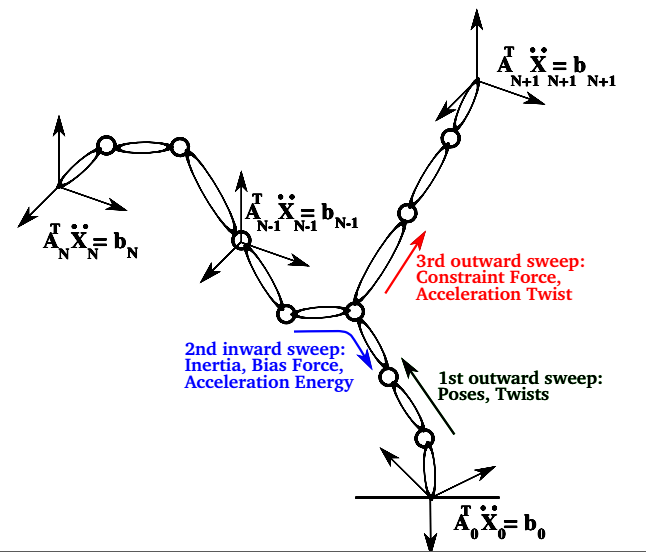
\includegraphics[scale=0.4]{images/solver_1}
	\caption{sweep}
\end{figure}\\
%The solver in different stages can be viewed as below: \\
\section{Comprehensive explanation of the solver}
In the sweeps, the variables q is represented as spatial position vector,$\dot{q}$ as spatial velocity vector, $\ddot{q}$ as spatial acceleration vector, $\tau_{a}$ as spatial force vector at each joint. These are represented using Plucker co-ordinates (mentioned in appendix\cite{shakhimardanov2015}.\\
\newpage
\textbf{Outward Sweep - Position, velocity, acceleration recursions}
\begin{enumerate}
	\item The beginning equation of this sweep indicates the calculation of pose relation between the links i+1 to i , i.e calculation of pose on proximal frames of segment i+1 w.r.t segment i. This is formed as the given equation as in\cite{shakhimardanov2015}:
	$$ {}^{i+1}_{i}X = compose({}^{d_i}_{i}X \ \  {}^{i+1}_{d_i}X(q_i))$$ 
	"This pose calculation is a composition of transformation ${}^{d_i}_{i}X$, between proximal/reference pose frame and distal frames/joint target of segment and transformation ${}^{i+1}_{d_i}X(q_i)$ between distal frame of link {i} and proximal frame of link {i+1}". These as indicated in the equation indicate that they are dependent on joint position qi.\cite{shakhimardanov2015}
	\item Inorder to find the spatial counterpart of $\dot{q}$ i.e, $\dot{X}$ of segment i+1 it requires joint velocity twist $\dot{X_{i}}$ contribution and also depends on joint velocity. The expression uses S which is the motion subspace matrix.(mention in appendix). Also the term ${}^{i+1}_{i}X$ indicates twist transformation matrix relating co-ordinates between i+1 and i.
	\item Similarly, given the joint velocity, joint rate and joint acceleration of segment {i+1}, the acceleration recursion calculates  the linear and angular components of bias acceleration $\ddot{X}_{i+1}$. The detailed expression uses the property of spatial cross product operator(mention in appendix). The above expression will only be calculated when joint acceleration is known, which is true only in case of inverse dynamics where forces/moments of force are computed with given desired segment motions. But in the case of forward dynamics , it is necessary to compute the desired motion of the segments, when the desired forces are given.\cite{shakhimardanov2015}
	\item Later, in the consecutive step the solver computes bias force, this is given by spatial vector of velocity cross product with inertial matrix and subtracted by external forces of segment i+1. The expression ${}^{i+1}_{0}X^*$ is a matrix representation of transformation between frames i+1 and i(mention in appendix) and $F^{ext}_{0,i+1}$ indicates that the measured force in frame i+1 is expressed in base frame(0).
%		
\end{enumerate}
\textbf{Inward force and inertia recursions}
\begin{enumerate}
	\item This deals with calculation of articulated body quantities such inertia and force vectors with rigid body quantities. The calculations are performed for each value of i from N-1 down 0.\cite{featherstone}. The equation ${D_{i+1} = d_{i+1} + S_{i+1}^T I_{i+1}^A S_{i+1} }$ is given as the transformed inertia. Also The term $S_{i+1}^T I_{i+1}^A S_{i+1}$ is positive definite matrix, and thus invertible. 
	\item The later step calculates the projection matrix of segment i+1, which deals with the projection of the inertias of the articulated body onto the joint axis. As mentioned above, the next steps indicate calculations of apparent inertias and are summed up from all children segments in the kinematic tree. Similarly, the apparent bias forces are summed up as transmitted by children segments as $F_{bias}^{a}$ which contributes to articulated body forces.
	\item The term $A$ is a unit constrained force matrix of dimension $6\times6$ matrix, and indicates to which direction is the acceleration constrained. These can be in linear and angular directions. But however, the magnitude of constraint forces are still unknown. 
	\item The subsequent stage represents the matrix $U$ which indicates the magnitude of forces that the solver is expected to calculate, which begins from end effector down to segment i. As mentioned in \cite{shakhimardanov2015}, the inward sweep monitors "...how much of desired constraint acceleration energy i.e, $b_{N}$" has already been generated by the $F_{ext}$ and also by the torques applied on joints.\cite{shakhimardanov2015}. 
	\item The expression 'L' is a $n\times n$ matrix called the constraint coupling matrix. This keeps monitoring the acceleration energy which has already been generated by the unit constraint force matrix. The matrices $U_{N}$ and $L_{N}$ are initialized to 0. Since the matrix is inverted, this matrix becomes rank deficient when the robot reaches the singular configuration. The basic solution present on the solver as a solution to singularity is damped least square method, which has been further evaluated as in (section implementation). As mentioned in the algorithm, the balance equation will allow computation of magnitude of constraint forces.	
\end{enumerate}
\textbf{Outward Sweep - torques, cartesian accelerations}
\begin{enumerate}
	\item The final recursion equation provides a relationship between torques and acceleration at the joint i+1. The resulting control torque is a combined effect of feed-forward torques, torques due to bias forces, and also torques generated due to constraint forces. Hence in forward dynamics the joint torques are known and thus the joint accelerations can be easily derived from the above equation.
	\item Finally, the cartesian acceleration is calculated/segment acceleration from the above results.
\end{enumerate}
\section{Constraint Specification}
This section explains the specification of constraints or how the task can be specified in Popov-vereshchagin solver. These tasks can be specified through constraints which are physical, virtual. The physical constraints for eg be contact with the environment\cite{shakhimardanov2015}.Virtual constraints being desired operational accelerations which are applied onto the segment/end effector.\cite{shakhimardanov2015}
The constraints which are specified on the end effector segment should fulfill this equation as in \cite{shakhimardanov2015} 
$$A_{N}^{T}\ddot{X}_{N} = b_{N}$$ 
The above equation is "linearly constrained"\cite{shakhimardanov2015}. Depending on the number of constraints(m) the dimension of matrix $A_{N}$ will be $6\times m$ which is called unit constrained force matrix and the matrix $b_{N}$ will be $m\times 1$ vector which is called acceleration energy. The columns of $A_{N}$ represent that the directions in which the segment is constrained. The constraints can be specified by the user, where it can be completely stated by the end user or partially stated in such a way that the they are less than m. For eg: constraining the motion of the end effector/segment in linear z and angular x directions, then we can define the unit constraint matrix to be \cite{shakhimardanov2015}
\[
\begin{bmatrix}
	A_{N} 
\end{bmatrix}
=
\begin{bmatrix}
	0 & 0 \\ 0 & 0 \\ 1 & 0 \\ 0 & 1 \\ 0 & 0 \\ 0 & 0
\end{bmatrix},
\begin{bmatrix}
b_{N}
\end{bmatrix}
=
\begin{bmatrix}
 0 \\ 0
\end{bmatrix}
\]
The first three rows of the constraint specification matrix allow to specify the linear constraints in x,y and z directions and similarly the lower three rows specify for angular constraints in the respective directions. These constraints indeed restrict the robot from achieving its motion in these directions, also acceleration energy has been set to zero which indicates the robot does not produce any acceleration energy in these particular directions. 
\par Lets consider another case where we can specify five constraints to the robot, i.e constraining all motions in a 5 DOF robot. The end effector/segment is allowed motion in all directions except in angular x as in \cite{shakhimardanov2015}
\[
\begin{bmatrix}
A_{N} 
\end{bmatrix}
=
\begin{bmatrix}
1 & 0 & 0 & 0 & 0 & 0\\ 0 & 1 & 0 & 0 & 0 & 0 \\ 0 & 0 & 1 & 0 & 0 & 0 \\ 0 & 0 & 0 & 0 & 0 & 0 \\0 & 0 & 0 & 0 & 1 & 0 \\ 0 & 0 & 0 & 0 & 0 & 1
\end{bmatrix},
\begin{bmatrix}
b_{N}
\end{bmatrix}
=
\begin{bmatrix}
0 \\ 0 \\ 0 \\0 \\0 \\0
\end{bmatrix}
\]
Finally, constraining all 6 directions of the end effector, we get an Identity matrix of size $6 \times 6$ as in \cite{shakhimardanov2015}
\[
\begin{bmatrix}
A_{N} 
\end{bmatrix}
=
\begin{bmatrix}
I_{6\times 6}
\end{bmatrix},
\begin{bmatrix}
b_{N}
\end{bmatrix}
=
\begin{bmatrix}
\ddot{X}_{N}
\end{bmatrix}
\]
Here, we assign the spatial acceleration vector to acceleration energy vector, even though they differ in their physical units. This signifies that the acceleration energy is produced by constraint forces which is dealt for each of the directional constraints. Hence, a single value specification in each individual columns of matrix $A_{N}$ suggest that the constraint force works only in that particular direction. "In turn follows that value of acceleration energy is the same as value of acceleration, in respective direction."\cite{Vuckevic}.